We begin by determination of the phases stable at a given temperature: initially 298K; These are determined by examining binary alloy phase diagrams for each of the possible element pairs, for example $Cu-Zn$, $Cu-Sn$, $Cu-S$ etc. 

After building a list of possible stable phases, we then produced four Ternary phase diagrams - at the vertices sit three of the four elements, and the edges of the diagram correspond to a varying percentage composition of the elements at either end of the line. 

On these edges, we mark the stable compounds and then draw from each compound a 'tie-line' to the element at the opposite vertex, and to each compound on the remaining edges. 

These tie-lines correspond to stable pairs of phases, and where these lines cross one another represents a reaction whereby one of the lines represents reactants, and the other the products. In order to determine which is more stable (the products), and as such which line should remain, we examine the Gibb's Free Energy of the reactants ($\Delta G_{r}^{\circ}$)\citep{perrot_z_1998} using the equation $\Delta G_{r}^{\circ} = \Sigma\Delta {G_{r}^{\circ}}_{products} - \Sigma\Delta {G_{r}^{\circ}}_{reactants}$ we can see which direction the reaction favours.

By finding the favoured direction, and as such the favoured tie-line, we can remove the other line, which will subsequently reduce the number of crossing points remaining. We then repeat this system of calculations on remaining crossing points, removing the unfavoured tie-lines until no more crossing points remain, leaving only a set of stable tie-lines.

We repeat this for each of the possible combinations of elements, producing four Ternary Phase Diagrams, each only having stable tie-lines. Using these, we can then produce a quaternary diagram, by joining each of the Ternary Diagrams and folding to produce a tetrahedron. 

Evident upon the tetrahedron will be the tie-lines from each of the respective Ternary Diagrams, which where they join on three surfaces will produce a 'tie-phase'. These tie-phases will be similar to the Ternary Diagrams, but rather than having elements at the vertices, it will have compounds.

We can look at each tie-plane, to see whether there are any crossing vectors with other tie-planes. If these occur we perform similar calculations to those performed for the tie-lines, and as such remove the unfavoured tie-plane.

We then subsequently either resolve each tie-plane in order to find one which provides the optimum thermodynamic conditions for production of $Cu_2ZnSnS_4$; or choose a tie-plane that has the correct proportions of the required elements, and subsequently resolve it to find the area that $Cu_2ZnSnS_4$ would occur, and the primary and secondary phases associated with it.

\begin{figure}
\centering
\begin{subfigure}{80mm}
  \centering
    \includegraphics[width=80mm]{triangleplot_ZNSNS298-before.png}
    \caption{Before Calculations}
    \label{fig:ZnSnSBefore}
\end{subfigure}%
\begin{subfigure}{80mm}
 \centering
    \includegraphics[width=80mm]{triangleplot_ZNSNS298.png}
    \caption{After Calculations}
    \label{fig:ZnSnS}
\end{subfigure}
\caption{Before and After Performing 'Tie-Line' Calculations. Percentage of each element run counter-clockwise.}
\label{fig:ZnSnSFigures}
\end{figure}

Subsequently, the method for removal of 'Tie-lines' is demonstrated, and Figure 1 demonstrates the difference before and after the calculations are completed.

\begin{enumerate}
\item For this point the balanced equation is $2 Zn + SnS_2 \rightarrow 2 ZnS + Sn$. $\Delta G_{r}^{\circ}$ for the reaction is found by: $\Delta G_{r}^{\circ} = (\Delta {G_{r}^{\circ}}_{ZnS} + \Delta {G_{r}^{\circ}}_{Sn}) - (\Delta {G_{r}^{\circ}}_{Zn} + \Delta {G_{r}^{\circ}}_{SnS_2})$. Using the data from the appendix, we find $\Delta G_{r}^{\circ}=(2x-201.3 + 0)-(-145.5+2x0)=$-257.1kJ $mol^{-1}$. Since the energy is found to be negative, the reaction moves left to right, as such we find that $ZnS$ and $Sn$ are in preference to $Zn$ and $SnS_2$. As such the $Zn$ and $SnS_2$ will be removed.


\item For this point the balanced equation is $ 3 ZnS + 2 Sn \rightarrow 3 Zn + Sn_2S_3$. $\Delta G_{r}^{\circ}$ for the reaction is found by $\Delta G_{r}^{\circ}=(2x0 -245.3)-(3x-201.3+2x0)=$+358.6kJ $mol^{-1}$. We use the same method of calculation here to find that the $ZnS$ and $Sn$ should be retained whilst the $Zn$ and $Sn_2S_3$ line discarded. 


\item For this point the balanced equation is $Zn + SnS \rightarrow ZnS + Sn$. $\Delta G_{r}^{\circ}$ for the reaction is found by: $\Delta G_{r}^{\circ}=(0+ -201.3)-(-98.3+0)$-257.1kJ $mol^{-1}$. Using the same method as before we find that the $ZnS$ and $Sn$ line should remain.
\item For this point the balanced equation is $Zn + SnS_2 \rightarrow ZnS + SnS$. However due to the removal of the lines in the previous calculations, this crossing point no longer exists, and as such no calculations are required.
\item For this point the balanced equation is $Zn + Sn_2S_3 \rightarrow ZnS + 2 SnS$. However due to the removal of the lines in the previous calculations, this crossing point no longer exists, and as such no calculations are required.
\item For this point the balanced equation is $Zn + 2 SnS_2 \rightarrow ZnS + Sn2S_3$. However due to the removal of the lines in the previous calculations, this crossing point no longer exists, and as such no calculations are required.
\end{enumerate}

Similar calculations were subsequently performed on the remaining faces of the tetrahedron - those being Cu-Zn-S, Cu-Zn-Sn, Cu-Sn-S, presented in section 3.

Upon completing calculations for each of the faces, it is apparent from the remaining 'Tie-lines' that some tie lines may form secondary 'Tie-phases' - Ternary phase Diagrams with compounds rather than elements at each vertice, with the edged of the diagram being 'Tie-lines' on the original diagrams. An example of these is shown below, and it is using these diagrams we will find the thermodynamic location of CZTS. By looking at each of the 'Tie-phases', we can  work out whether CZTS will exist along that phase by looking at the ratio of elements in the compounds, upon finding such a phase we can find the general location of CZTS using the atomic percentages of the elements. An example of the 'Tie-phase' is demonstrated in Figure 2, and a solved phase is present in the Results section.

\begin{figure}
\centering
\begin{subfigure}{80mm}
 \centering
    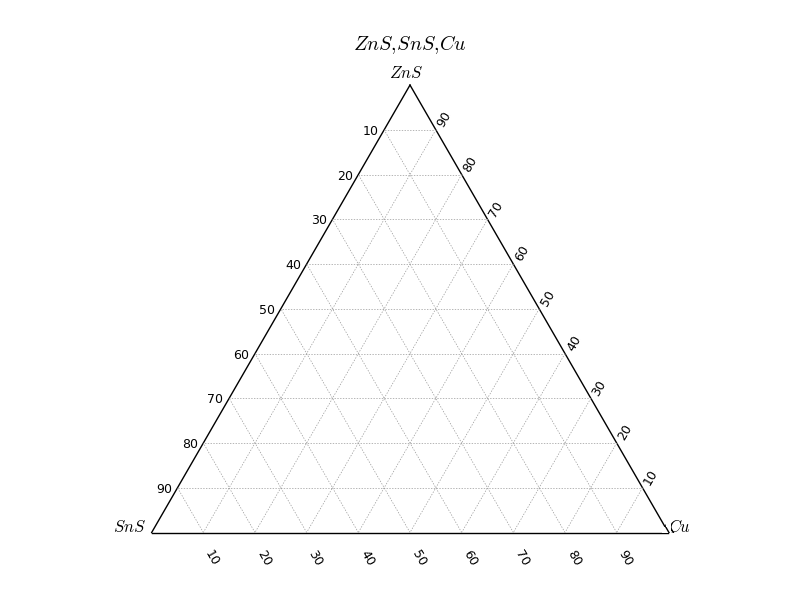
\includegraphics[width=80mm]{triangleplot_ZnSSnSCu298.png}
    \caption{Percentages of ZnS, SnS, Cu running counter-clockwise}
    \label{fig:ZnSSnSCu}
\end{subfigure}%
\caption{Dismissed tie Phase Diagram, without associated phases}
\label{fig:ZnSSnSCuFig}
\end{figure}

